\documentclass[times, utf8, seminar, numeric]{fer}
\usepackage{booktabs}
 \usepackage{url}
 \usepackage{tikz}
 \usepackage{todonotes}
 \usepackage[onelanguage,croatian,croatiankw]{algorithm2e}
 
 
 \usetikzlibrary{matrix}
 %\usetikzlibrary{external}
 %\tikzexternalize[prefix=build/]
 
 

\begin{document}

% Ukljuci literaturu u seminar
\nocite{*}

\title{Pronalazak najkraćeg puta algoritmom A*}

\author{Marko Lazarić}

\voditelj{Doc. dr. sc. Marko Čupić}

\maketitle

\tableofcontents

\chapter{Uvod}
Velik broj problema može se modelirati grafom u kojem vrhovi predstavljaju stanja, a bridovi prijelaze između tih stanja, takav graf se naziva prostor stanja \engl{state space}.
Rješavanje problema se onda svodi na pretraživanje prostora stanja, odnosno pronalazak najkraćeg puta između početnog stanja i stanja koje predstavlja rješenje problema.

% Problem pronalaska najkraćeg puta između dva vrha u grafu jedan je od najstarijih i najbolje istraženih problema u teoriji grafova. Rješenja tog problema imaju široku primjenu jer se velik broj situacija u pravom svijetu može modelirati kao grafovi, gdje vrhovi predstavljaju stanja, a bridovi prijelaze između tih stanja. Provedbom ovih algoritama minimizira se broj prijelaza, odnosno trošak za prijelaz od početnog do završnog stanja.

Zbog svoje široke primjenjivosti, osmišljeni su razni algoritmi za efikasno rješavanje tog problema. U ovom seminaru razmatrat će se prednosti i mane različitih algoritama za pronalazak najkraćeg puta između dva vrha u grafu, počevši od jednostavnijih naivnih algoritama,  do složenijih za implementaciju, ali efikasnijih informiranih algoritama s naglaskom na algoritam A* i njegovu primjenu na pronalazak najkraćeg puta u cjelobrojnoj rešetci. 

U svrhu jednostavne vizualizacije rada algoritama, koristit će se cjelobrojna rešetka u kojoj sivi kvadratići predstavljaju neprolazna polja, dok bijeli predstavljaju polja kroz koja se može proći. Moguće je kretati se u 4 osnovna smjera. "A" predstavlja početno stanje (vrh), a "B" završno. 

\begin{figure}[h]
	\centering
	
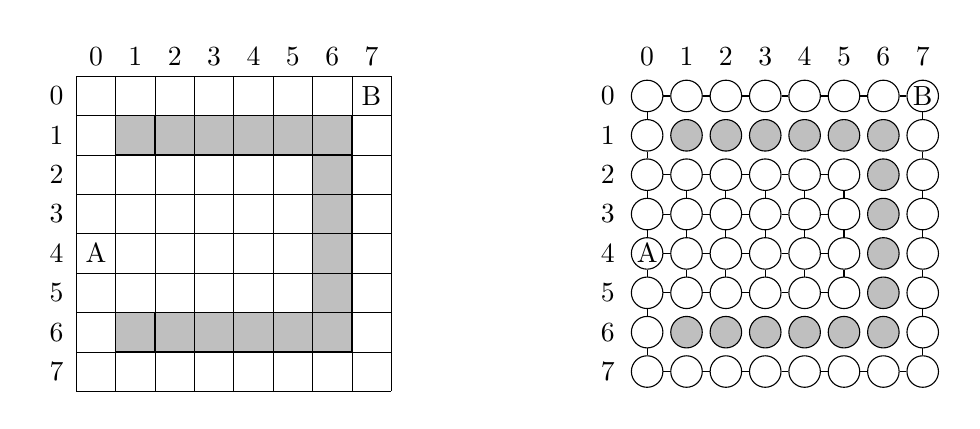
\begin{tikzpicture}
	\begin{scope}
		\begin{scope}[xshift=0.25cm, yshift=-0.25cm]
	\draw[step=0.5cm,black,very thin] (-2,-2) grid (2,2);
	
	\newcommand\fillSquare[2]{\filldraw[fill=lightgray] (#1 / 2,#2 / 2) rectangle (#1 / 2 + 0.5,#2 / 2 + 0.5)}
	
	
	\foreach \x in {-3,...,2}
	{
		\fillSquare{\x}{-3};
		\fillSquare{\x}{2};
		\fillSquare{2}{\x};
	}
\end{scope}

\matrix[matrix, matrix of nodes, nodes={anchor=center,inner sep=0pt,text width=.5cm,align=center,minimum height=.5cm}, nodes in empty cells]{
& 0 & 1 & 2 & 3 & 4 & 5 & 6 & 7 \\
 0 &   &   &   &   &   &   &   & B \\
	1 &   &   &   &   &   &   &   &   \\
	2 &   &   &   &   &   &   &   &   \\
	3 &   &   &   &   &   &   &   &   \\
	4 & A &   &   &   &   &   &   &   \\
	5 &   &   &   &   &   &   &   &   \\
	6 &   &   &   &   &   &   &   &   \\
	7 &   &   &   &   &   &   &   &   \\};
	\end{scope}
	
	\begin{scope}[xshift=7cm]
	    \matrix[matrix, matrix of nodes, nodes={anchor=center,inner sep=0pt,text width=.5cm,align=center,minimum height=.5cm}, nodes in empty cells]{
   	& 0 & 1 & 2 & 3 & 4 & 5 & 6 & 7 \\
   	0 &   &   &   &   &   &   &   &   \\
   	1 &   &   &   &   &   &   &   &   \\
   	2 &   &   &   &   &   &   &   &   \\
   	3 &   &   &   &   &   &   &   &   \\
   	4 &   &   &   &   &   &   &   &   \\
   	5 &   &   &   &   &   &   &   &   \\
   	6 &   &   &   &   &   &   &   &   \\
   	7 &   &   &   &   &   &   &   &   \\};
  	
\newcommand\drawNode[4]{\node[circle,draw,inner sep=0pt,minimum size=0.4cm] at (#1 / 2 - 1.5, #2 / 2 - 2)   (#4) {#3};}
\newcommand\drawWallNode[3]{\node[circle,draw,fill=lightgray,inner sep=0pt,minimum size=0.4cm] at (#1 / 2 - 1.5, #2 / 2 - 2)   (#3) {};}

\drawNode{0}{0}{ }{0}
\drawNode{1}{0}{ }{1}
\drawNode{2}{0}{ }{2}
\drawNode{3}{0}{ }{3}
\drawNode{4}{0}{ }{4}
\drawNode{5}{0}{ }{5}
\drawNode{6}{0}{ }{6}
\drawNode{7}{0}{ }{7}
\drawNode{0}{1}{ }{8}
\drawWallNode{1}{1}{9}
\drawWallNode{2}{1}{10}
\drawWallNode{3}{1}{11}
\drawWallNode{4}{1}{12}
\drawWallNode{5}{1}{13}
\drawWallNode{6}{1}{14}
\drawNode{7}{1}{ }{15}
\drawNode{0}{2}{ }{16}
\drawNode{1}{2}{ }{17}
\drawNode{2}{2}{ }{18}
\drawNode{3}{2}{ }{19}
\drawNode{4}{2}{ }{20}
\drawNode{5}{2}{ }{21}
\drawWallNode{6}{2}{22}
\drawNode{7}{2}{ }{23}
\drawNode{0}{3}{A}{24}
\drawNode{1}{3}{ }{25}
\drawNode{2}{3}{ }{26}
\drawNode{3}{3}{ }{27}
\drawNode{4}{3}{ }{28}
\drawNode{5}{3}{ }{29}
\drawWallNode{6}{3}{30}
\drawNode{7}{3}{ }{31}
\drawNode{0}{4}{ }{32}
\drawNode{1}{4}{ }{33}
\drawNode{2}{4}{ }{34}
\drawNode{3}{4}{ }{35}
\drawNode{4}{4}{ }{36}
\drawNode{5}{4}{ }{37}
\drawWallNode{6}{4}{38}
\drawNode{7}{4}{ }{39}
\drawNode{0}{5}{ }{40}
\drawNode{1}{5}{ }{41}
\drawNode{2}{5}{ }{42}
\drawNode{3}{5}{ }{43}
\drawNode{4}{5}{ }{44}
\drawNode{5}{5}{ }{45}
\drawWallNode{6}{5}{46}
\drawNode{7}{5}{ }{47}
\drawNode{0}{6}{ }{48}
\drawWallNode{1}{6}{49}
\drawWallNode{2}{6}{50}
\drawWallNode{3}{6}{51}
\drawWallNode{4}{6}{52}
\drawWallNode{5}{6}{53}
\drawWallNode{6}{6}{54}
\drawNode{7}{6}{ }{55}
\drawNode{0}{7}{ }{56}
\drawNode{1}{7}{ }{57}
\drawNode{2}{7}{ }{58}
\drawNode{3}{7}{ }{59}
\drawNode{4}{7}{ }{60}
\drawNode{5}{7}{ }{61}
\drawNode{6}{7}{ }{62}
\drawNode{7}{7}{B}{63}
\draw[] (0) -- (8);
\draw[] (0) -- (1);
\draw[] (1) -- (2);
\draw[] (1) -- (0);
\draw[] (2) -- (3);
\draw[] (2) -- (1);
\draw[] (3) -- (4);
\draw[] (3) -- (2);
\draw[] (4) -- (5);
\draw[] (4) -- (3);
\draw[] (5) -- (6);
\draw[] (5) -- (4);
\draw[] (6) -- (7);
\draw[] (6) -- (5);
\draw[] (7) -- (15);
\draw[] (7) -- (6);
\draw[] (8) -- (16);
\draw[] (8) -- (0);
\draw[] (15) -- (23);
\draw[] (15) -- (7);
\draw[] (16) -- (24);
\draw[] (16) -- (8);
\draw[] (16) -- (17);
\draw[] (17) -- (25);
\draw[] (17) -- (18);
\draw[] (17) -- (16);
\draw[] (18) -- (26);
\draw[] (18) -- (19);
\draw[] (18) -- (17);
\draw[] (19) -- (27);
\draw[] (19) -- (20);
\draw[] (19) -- (18);
\draw[] (20) -- (28);
\draw[] (20) -- (21);
\draw[] (20) -- (19);
\draw[] (21) -- (29);
\draw[] (21) -- (20);
\draw[] (23) -- (31);
\draw[] (23) -- (15);
\draw[] (24) -- (32);
\draw[] (24) -- (16);
\draw[] (24) -- (25);
\draw[] (25) -- (33);
\draw[] (25) -- (17);
\draw[] (25) -- (26);
\draw[] (25) -- (24);
\draw[] (26) -- (34);
\draw[] (26) -- (18);
\draw[] (26) -- (27);
\draw[] (26) -- (25);
\draw[] (27) -- (35);
\draw[] (27) -- (19);
\draw[] (27) -- (28);
\draw[] (27) -- (26);
\draw[] (28) -- (36);
\draw[] (28) -- (20);
\draw[] (28) -- (29);
\draw[] (28) -- (27);
\draw[] (29) -- (37);
\draw[] (29) -- (21);
\draw[] (29) -- (28);
\draw[] (31) -- (39);
\draw[] (31) -- (23);
\draw[] (32) -- (40);
\draw[] (32) -- (24);
\draw[] (32) -- (33);
\draw[] (33) -- (41);
\draw[] (33) -- (25);
\draw[] (33) -- (34);
\draw[] (33) -- (32);
\draw[] (34) -- (42);
\draw[] (34) -- (26);
\draw[] (34) -- (35);
\draw[] (34) -- (33);
\draw[] (35) -- (43);
\draw[] (35) -- (27);
\draw[] (35) -- (36);
\draw[] (35) -- (34);
\draw[] (36) -- (44);
\draw[] (36) -- (28);
\draw[] (36) -- (37);
\draw[] (36) -- (35);
\draw[] (37) -- (45);
\draw[] (37) -- (29);
\draw[] (37) -- (36);
\draw[] (39) -- (47);
\draw[] (39) -- (31);
\draw[] (40) -- (48);
\draw[] (40) -- (32);
\draw[] (40) -- (41);
\draw[] (41) -- (33);
\draw[] (41) -- (42);
\draw[] (41) -- (40);
\draw[] (42) -- (34);
\draw[] (42) -- (43);
\draw[] (42) -- (41);
\draw[] (43) -- (35);
\draw[] (43) -- (44);
\draw[] (43) -- (42);
\draw[] (44) -- (36);
\draw[] (44) -- (45);
\draw[] (44) -- (43);
\draw[] (45) -- (37);
\draw[] (45) -- (44);
\draw[] (47) -- (55);
\draw[] (47) -- (39);
\draw[] (48) -- (56);
\draw[] (48) -- (40);
\draw[] (55) -- (63);
\draw[] (55) -- (47);
\draw[] (56) -- (48);
\draw[] (56) -- (57);
\draw[] (57) -- (58);
\draw[] (57) -- (56);
\draw[] (58) -- (59);
\draw[] (58) -- (57);
\draw[] (59) -- (60);
\draw[] (59) -- (58);
\draw[] (60) -- (61);
\draw[] (60) -- (59);
\draw[] (61) -- (62);
\draw[] (61) -- (60);
\draw[] (62) -- (63);
\draw[] (62) -- (61);
\draw[] (63) -- (55);
\draw[] (63) -- (62);
		
			
			
	\end{scope}
\end{tikzpicture}
	\caption{Primjer jednostavne cjelobrojne rešetke i njezinog prostora stanja.} 
\end{figure}




\section{Definicija problema}
Opisani problem definiran je s pet komponenata \cite{russelNorvig2003:aima}:

\begin{enumerate}
	\item početno stanje \engl{initial state}, 
	\item moguće akcije \engl{actions} -- opis mogućih akcija u nekom stanju,
	\item model prijelaza \engl{transition model} -- opis što svaka akcija znači, 
	\item provjera riješenosti \engl{goal test} -- provjera je li neko stanje rješenje te
	\item funkcija troška prijelaza između stanja \engl{step cost}.
\end{enumerate}

Za problem cjelobrojne rešetke, početno stanje je stanje sa slovom "A".
Moguće akcije su: gore, dolje, lijevo i desno.
Model prijelaza je intuitivan: gore povećava y koordinatu za jedan, dolje ju smanjuje, a lijevo i desno povećavaju, odnosno smanjuju x koordinatu.
Provjera riješenosti provjerava sadrži li stanje slovo "B".
Trošak neposrednog prijelaza između stanja je uvijek jednak 1.
Definicija tog problema implementirana je razredom \texttt{RectangularGrid}.
\section{Kriteriji uspoređivanja algoritama}
Algoritme za rješavanje navedenog problema možemo uspoređivati po 4 kriterija \cite{russelNorvig2003:aima}:

\begin{enumerate}
	\item Potpunost -- potpuni algoritam će uvijek pronaći rješenje, ako rješenje postoji.
	\item Optimalnost -- optimalni algoritam će uvijek pronaći optimalno rješenje, ako rješenje postoji.
	\item Vremenska složenost -- koliko dugo traje izvođenje algoritma u ovisnosti s veličinom ulaza.
	\item Memorijska složenost -- koliko memorije treba algoritam u ovisnosti s veličinom ulaza.
\end{enumerate}

Pri analizi vremenske i memorijske složenosti korisne su sljedeće oznake: \( b \) faktor grananja (najveći broj sljedbenika iz nekog stanja), \( d \) dubina rješenja s najmanjom dubinom i \( m \) najveća duljina bilo kojeg puta u prostoru stanja.

\chapter{Naivni algoritmi}
Naivni algoritmi \engl{uniformed algorithms} nemaju dodatne informacije o stanjima, pa smatraju da svaki prijelaz ima jednaku vjerojatnost da dovede do najkraćeg puta. 
Njihove prednosti su jednostavna implementacija i generalnost, a mana im je velika memorijska i vremenska složenost. 


\section{Pretraživanje u širinu}
Pretraživanje u širinu \engl{breadth-first search} je jednostavan algoritam za pronalazak najkraćeg puta u grafu s uniformnim težinama bridova.
Algoritam je potpun i optimalan, a njegova vremenska i memorijska složenost je \( O(b^d) \). \cite{russelNorvig2003:aima}

Za pohranu vrhova koje treba obraditi koristi red \engl{queue}, dok za pohranu već obrađenih vrhova koristi skup \engl{set}.
U svakom koraku širi se u svim mogućim smjerovima, što dovodi do velike memorijske i vremenske složenosti.
Implementiran je metodom \texttt{bfs} u razredu \texttt{SearchAlgorithms}.

\begin{algorithm}[h]
	fronta $\gets$ FIFO red vrhova s jednim elementom: (pocetnoStanje, null, 0)\;
	pronadeni $\gets$ skup s jednim elementom: pocetnoStanje\;
	\While{fronta nije prazna}{
		trenutni $\gets$ prvi element iz fronte\;
		\eIf{trenutni.stanje je rjesenje}{
			vrati trenutni\;
		}{
			prijelazi $\gets$ prijelazi iz trenutni.stanje\;
			\ForEach{prijelaz iz prijelazi}{
				\If{prijelaz.stanje nije u pronadeni}{
					dodaj prijelaz.stanje u pronadeni\;
					dodaj (prijelaz.stanje, trenutni, trenutni.cijena + prijelaz.cijena) u frontu\;
				}
			}
		}
	}
	vrati null\;
	\caption{Pseudokod pretraživanja u širinu.}
\end{algorithm}

Na slici \ref{inefficient_bfs} je prikazano izvođenje algoritma.
Crvenom bojom su označena polja koje je algoritam obradio, ali nisu dovela do najkraćeg puta, dok je zelenom označen najkraći put.
Brojevi u poljima označavaju udaljenost od početnog polja.
Pretraga u širinu je obradila \( 41 \) polja, dok bi optimalno rješenje obradilo samo \( 8 \). 

\begin{figure}[h]
	\centering
	\begin{tikzpicture}
		\begin{scope}
			\input{figures/bfs.tex}
		\end{scope}
		
		\begin{scope}[xshift = 7.5cm]
			\input{figures/optimal.tex}
		\end{scope}
	\end{tikzpicture}
	\caption{Usporedba pretraživanja u širinu i optimalnog rješenja.} 
	\label{inefficient_bfs}
\end{figure}

\clearpage
\section{Pretraživanje s jednolikom cijenom}
Pretraživanje s jednolikom cijenom \engl{uniform-cost search} je jednostavan algoritam za pronalazak najkraćeg puta u grafu s pozitivnim težinama bridova.
Algoritam je potpun i optimalan, a njegova vremenska i memorijska složenost je \( O \left (b^{1 + \lfloor {C^*}/{\epsilon} \rfloor} \right ) \) gdje \( C^* \) predstavlja cijenu optimalnog rješenja, a \( \epsilon \) minimalnu težinu svih bridova. \cite{russelNorvig2003:aima}

Za pohranu vrhova koristi prioritetni red \engl{priority queue}, te hash tablicu radi efikasne provjere je li pronašao bolji put do nekog vrha koji se već nalazi u prioritetnom redu.
Implementiran je metodom \texttt{ucs} u razredu \texttt{SearchAlgorithms}.

Prioritetni red koristi evaluacijsku funkciju \engl{evaluation function} za određivanje prioriteta, pri tome se manji broj smatra većim prioritetom. 
Označava se s \( f(n) \).
Konkretno za pretraživanje s jednolikom cijenom evaluacijska funkcija je jednaka cijenom puta od početnog vrha do tog vrha. 
Oznaka za cijenu puta od početka do tog vrha je \( g(n) \), pa za pretraživanje s jednolikom cijenom vrijedi \( f(n) = g(n) \).

\todo[inline]{Pseudokod}

Za grafove s uniformnim težinama bridova, pretraživanje s jednolikom cijenom obradi strogo više vrhova od pretraživanja u širinu jer provjerava je li vrh rješenje pri obradi vrha.
Posljedica toga je da algoritam obrađuje sve vrhove koji imaju istu cijenu, prije nego što obradi njihove sljedbenike.

\begin{figure}[h]
	\centering
	\begin{tikzpicture}
		\begin{scope}
			\input{figures/bfs.tex}
		\end{scope}
		
		\begin{scope}[xshift = 7.5cm]
			
\begin{scope}[xshift=0.25cm, yshift=-0.25cm]
	\fill[fill = green!10] (-2, -0.5) rectangle (2, 0);
	
	\path[fill = red!10] (-2, -0.5) -- (1.5, -0.5) -- (1.5, -1) -- (1, -1) -- (1, -1.5) -- (0.5, -1.5) -- (0.5, -2) -- (-2, -2) -- cycle;
	
	\path[fill = red!10] (-2, 0) -- ++(0, 2) -- ++(2, 0) -- ++(0, -0.5) -- ++(0.5, 0) -- ++(0, -0.5) -- ++(0.5, 0) -- ++(0, -0.5) -- ++(0.5, 0) -- ++(0, -0.5) -- cycle;
	
	\draw[step=0.5cm,black,very thin] (-2,-2) grid (2,2);
\end{scope}

\matrix[matrix, matrix of nodes, nodes={anchor=center,inner sep=0pt,text width=.5cm,align=center,minimum height=.5cm}, nodes in empty cells]{
	  & 0 & 1 & 2 & 3 & 4 & 5 & 6 & 7 \\
	0 & 4 & 5 & 6 & 7 &   &   &   &   \\
	1 & 3 & 4 & 5 & 6 & 7 &   &   &   \\
	2 & 2 & 3 & 4 & 5 & 6 & 7 &   &   \\
	3 & 1 & 2 & 3 & 4 & 5 & 6 & 7 &   \\
	4 & A & 1 & 2 & 3 & 4 & 5 & 6 & B \\
	5 & 1 & 2 & 3 & 4 & 5 & 6 & 7 &   \\
	6 & 2 & 3 & 4 & 5 & 6 & 7 &   &   \\
	7 & 3 & 4 & 5 & 6 & 7 &   &   &   \\
};
		\end{scope}
	\end{tikzpicture}
	\caption{Usporedba pretraživanja u širinu i pretraživanja s jednolikom cijenom.} 
	\label{inefficient_ucs}
\end{figure}

\chapter{Informirani algoritmi}
Informirani algoritmi \engl{informed algorithms} koriste dodatne informacije o problemu kako bi smanjili prostor stanja kojeg trebaju pretražiti. 
Te informacije se najčešće ugrađuju u heurističku funkciju \engl{heuristic function} koja se označava s \( h(n) \), a predstavlja aproksimaciju najmanje cijene prijelaza od stanja \( n \) do stanja koje predstavlja rješenje.
Njihova prednost je manja memorijska i vremenska složenost, a mana im je specijalizacija za pojedini problem.
\section{Heuristička funkcija}
Heuristika \( h(n) \) je optimistična ili dopustiva ako i samo ako nikada ne precjenjuje cijenu puta od stanja \( n \) do cilja. Odnosno za svako stanje \( n \) vrijedi da je \( h(n) \) manje ili jednako od cijene optimalnog puta od stanja \( n \) do cilja. \cite{umjetna}

Heuristika \( h(n) \) je konzistentna ili monotona ako i samo ako za svako stanje \( n \) i za svaki njegov sljedbenik \( n' \) vrijedi: \( h(n) \leq c(n, n') + h(n') \) gdje \( c(n, n') \) predstavlja trošak prijelaza iz stanja \( n \) u stanje \( n' \). \cite{russelNorvig2003:aima}

Stanja u cjelobrojnoj rešetci označena su s dva cijela broja \( x \) i \( y \), pa se heuristička funkcija može zapisati kao \( h(x, y) \).
Neka je početno stanje \( A(x_A, y_A) \), a završno stanje \( B(x_B, y_B) \).
Onda se heuristička funkcija može definirati kao Manhattan udaljenost između trenutnog stanja i završnog, odnosno \( h(x, y) = |x - x_B| + |y - y_B| \).
Takva heuristička funkcija predstavlja najmanji broj prijelaza potrebnih za prijelaz iz trenutnog stanja u završno stanje, pa je nužno optimistična, a također je konzistentna.


\section{Pretraživanje "najbolji prvi"}
Pretraživanje "najbolji prvi" \engl{greedy best-first-search} je jednostavan pohlepan informiran algoritam koji nije optimalan, a potpun je jedino ako koristimo listu posjećenih stanja. \cite{russelNorvig2003:aima} \cite{umjetna}

Algoritam je ekvivalentan pretraživanju s jednolikom cijenom, osim što za evaluacijsku funkciju koristi heurističku funkciju \( f(n) = h(n) \).
To znači da će prvo evaluirati stanja koja su bliža rješenju, no taj lokalni optimum neće nužno dovesti do optimalnog rješenja, kao što je prikazano na slici \ref{greedy}.

\begin{figure}[h]
	\centering
	\begin{tikzpicture}
		\begin{scope}
			\input{figures/greedy_line.tex}
		\end{scope}
		
		\begin{scope}[xshift = 7.5cm]
			\begin{scope}[xshift=-1.75cm, yshift=1.75cm, xscale=0.5, yscale=0.5]
	\fill[fill = lightgray] (1, -1) -- ++(6, 0) -- ++(0, -6) -- ++(-6, 0) -- ++(0, 1) -- ++(5, 0) -- ++(0, 4) -- ++(-5, 0) -- cycle;
	
	\fill[fill = green!10] (0, -5)
	  -- ++(0, 1)
	  -- ++(5, 0)
	  -- ++(0, 1)
	  -- ++(-5, 0)
	  -- ++(0, 3)
	  -- ++(8, 0)
	  -- ++(0, -1)
	  -- ++(-7, 0)
	  -- ++(0, -1)
	  -- ++(5, 0)
	  -- ++(0, -3)
	  -- cycle;
	  
	\fill[fill = red!10] (1, -4)
	  -- ++(0, 1)
	  -- ++(4, 0)
	  -- ++(0, -1)
	  -- cycle;
	  
	\fill[fill = red!10] (3, -6)
	  -- ++(0, 1)
	  -- ++(3, 0)
  	  -- ++(0, -1)
	  -- cycle;
\end{scope}

\begin{scope}[xshift=0.25cm, yshift=-0.25cm]	
	\draw[step=0.5cm,black,very thin] (-2,-2) grid (2,2);
\end{scope}

\matrix[matrix, matrix of nodes, nodes={anchor=center,inner sep=0pt,text width=.5cm,align=center,minimum height=.5cm}, nodes in empty cells]{
	  & 0 & 1 & 2 & 3 & 4 & 5 & 6 & 7 \\
	0 & 14 & 15 & 16 & 17 & 18 & 19 & 20 & B \\
	1 & 13 &   &   &   &   &   &   &   \\
	2 & 12 & 11 & 10 & 9 & 8 & 7 &   &   \\
	3 &   & 8 & 5 & 6 & 9 & 6 &   &   \\
	4 & A & 1 & 2 & 3 & 4 & 5 &   &   \\
	5 &   &   &   & 4 & 7 & 6 &   &   \\
	6 &   &   &   &   &   &   &   &   \\
	7 &   &   &   &   &   &   &   &   \\
};
		\end{scope}
	\end{tikzpicture}
	\caption{Rezultat pohlepnog pretraživanja.} 
	\label{greedy}
\end{figure}
\section{Algoritam A*}
Algoritam A* je ekvivalentan pretraživanju s jednolikom cijenom, osim što za evaluacijsku funkciju koristi sumu cijene puta od početka do tog vrha i heurističke funkcije \( f(n) = g(n) + h(n) \). 
A* je uvijek potpun, a optimalan je pod uvjetom da je heuristika \( h(n) \) optimistična.
Vremenska i memorijska složenost mu je \( O \left (\textrm{min}(b^{d + 1}, b|S|) \right ) \). \cite{russelNorvig2003:aima} \cite{umjetna}

Heuristika \( h(n) \) je optimistična ili dopustiva \engl{optimistic, admissible} ako i samo ako nikada ne precjenjuje, odnosno ako nikada nije veća od prave cijene do cilja. \cite{umjetna}

\begin{figure}[h]
	\centering
	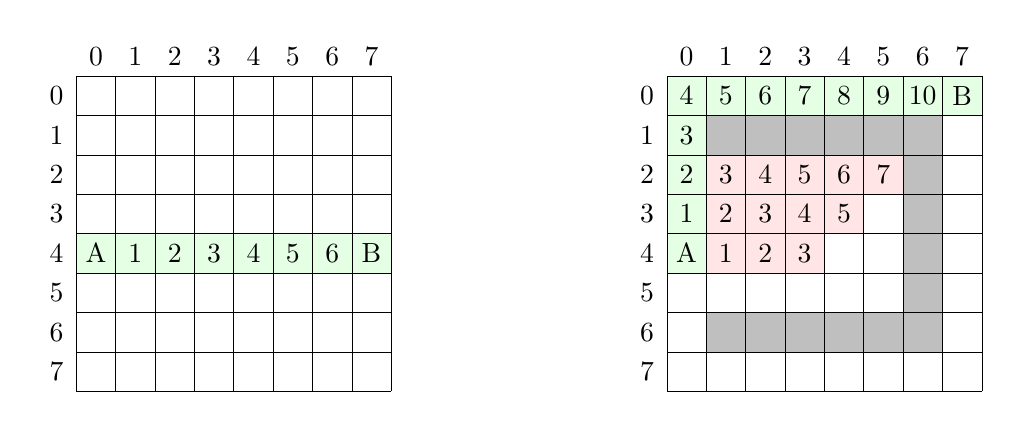
\begin{tikzpicture}
		\begin{scope}
			\begin{scope}[xshift=0.25cm, yshift=-0.25cm]
	\fill[fill = green!10] (-2, -0.5) rectangle (2, 0);
	
	\draw[step=0.5cm,black,very thin] (-2,-2) grid (2,2);
\end{scope}

\matrix[matrix, matrix of nodes, nodes={anchor=center,inner sep=0pt,text width=.5cm,align=center,minimum height=.5cm}, nodes in empty cells]{
	& 0 & 1 & 2 & 3 & 4 & 5 & 6 & 7 \\
	0 &   &   &   &   &   &   &   &   \\
	1 &   &   &   &   &   &   &   &   \\
	2 &   &   &   &   &   &   &   &   \\
	3 &   &   &   &   &   &   &   &   \\
	4 & A & 1 & 2 & 3 & 4 & 5 & 6 & B \\
	5 &   &   &   &   &   &   &   &   \\
	6 &   &   &   &   &   &   &   &   \\
	7 &   &   &   &   &   &   &   &   \\
};
		\end{scope}
		
		\begin{scope}[xshift = 7.5cm]
			\begin{scope}[xshift=-1.75cm, yshift=1.75cm, xscale=0.5, yscale=0.5]
	\fill[fill = lightgray] (1, -1) -- ++(6, 0) -- ++(0, -6) -- ++(-6, 0) -- ++(0, 1) -- ++(5, 0) -- ++(0, 4) -- ++(-5, 0) -- cycle;
	
	\fill[fill = green!10] (1, -5)
	  -- ++(-1, 0)
	  -- ++(0, 5)
	  -- ++(8, 0)
	  -- ++(0, -1)
	  -- ++(-7, 0)
	  -- cycle;
	  
	\fill[fill = red!10] (1, -5)
	  -- ++(0, 3)
	  -- ++(5, 0)
	  -- ++(0, -1) -- ++(-1, 0)
	  -- ++(0, -1) -- ++(-1, 0)
	  -- ++(0, -1) -- ++(-1, 0)
	  -- cycle;
\end{scope}

\begin{scope}[xshift=0.25cm, yshift=-0.25cm]	
	\draw[step=0.5cm,black,very thin] (-2,-2) grid (2,2);
\end{scope}

\matrix[matrix, matrix of nodes, nodes={anchor=center,inner sep=0pt,text width=.5cm,align=center,minimum height=.5cm}, nodes in empty cells]{
	  & 0 & 1 & 2 & 3 & 4 & 5 & 6 & 7 \\
	0 & 4 & 5 & 6 & 7 & 8 & 9 & 10 & B \\
	1 & 3 &   &   &   &   &   &   &   \\
	2 & 2 & 3 & 4 & 5 & 6 & 7 &   &   \\
	3 & 1 & 2 & 3 & 4 & 5 &   &   &   \\
	4 & A & 1 & 2 & 3 &   &   &   &   \\
	5 &   &   &   &   &   &   &   &   \\
	6 &   &   &   &   &   &   &   &   \\
	7 &   &   &   &   &   &   &   &   \\
};
		\end{scope}
	\end{tikzpicture}
	\caption{Rezultat algoritma A*.} 
	\label{astar}
\end{figure}

%\chapter{Primjena u cjelobrojnoj rešetci}
%\input{chapters/04_rectangular_grid.tex}

\chapter{Zaključak}
Algoritam A* je jednostavan informirani algoritam koji efikasno pretražuje prostor stanja uz dobro definiranu heurističku funkciju.
Njegova prednost je smanjenje prostora stanja koje treba pretražiti pomoću heurističke funkcije, no njegova mana je velika memorijska složenost, pa je običan A* primjenjiv prostore stanja.
Za istraživanje prostora stanja s velikim brojem stanja, prikladniji su algoritmi IDA* i SMA*.


\bibliography{literatura}
\bibliographystyle{fer}

\chapter{Sažetak}
Brojni problemi se mogu prikazati skupom stanja i prijelazima između njih, odnosno prostorom stanja. 
Rješavanje problema se svodi na istraživanje prostora stanja, te pronalazak najkraćeg puta iz nekog početnog stanja, do stanja koje predstavlja rješenje.

Postoje različiti algoritmi za istraživanje prostora stanja. 
Naivni algoritmi istražuju prostor stanja naivno, bez dodatnih informacija o problemu, što dovodi do velike vremenske i memorijske složenosti.

Informirani algoritmi koriste dodatne informacije kako bi smanjili prostor stanja koji trebaju istražiti.
Te dodatne informacije se ugrađuju u heurističku funkciju koja predstavlja aproksimaciju najmanje cijene prijelaza od stanja \( n \) do stanja koje predstavlja rješenje.
Prednost informiranih algoritama je manja vremenska i memorijska složenost zato što ne moraju istražiti cijeli prostor stanja.

Algoritam A* je informirani algoritam za pretraživanje prostora stanja koji kombinira heurističku funkciju i trenutnu cijenu kako bi smanjio prostor stanja kojeg treba istražiti, ali svejedno našao optimalno rješenje.
Postoje varijante algoritma A* koje nastoje smanjiti memorijsku složenost kao što su IDA* i SMA*.

U ovom seminaru opisane su obje kategorije algoritama, i naivni i informirani, prikazane su njihove razlike, kako u implementaciji, tako i u memorijskoj i vremenskoj složenosti. Osim same analize algoritama, vizualizacijama je pobliže objašnjen način rada, kao i slučajevi u kojima opisani algoritmi ne daju dobre rezultate.

\end{document}
